\chapterimage{images/intents/intentchapterimage.jpg}

\chapter{Intents and Broadcastreceivers}

\section{Intent}
Intents are objects which you can use for the following actions:


\begin{itemize}
	\item Explicitly start a particular Service or Activity using its class name (already seen in previous lessons)
	\item Implicitly start a particular Service or Activity
	\item Start an Activity or Service to perform an action with (or on) a particular piece of data
	\item Broadcast that an event has occurred
\end{itemize}

The two most important pieces of an Intent are the action and what Android refers
to as the data. If you were to create an Intent combining ACTION\_VIEW with a content Uri of
https://google.com , and pass that Intent to Android via startActivity() ,
Android would know to find and open an activity capable of viewing that resource.


There are other criteria you can place inside an Intent
\begin{description}
	\item[Categories] A string containing additional information about the kind of component that should handle the intent. Any number of category descriptions can be placed in an intent, but most intents do not require a category. Your “main” activity will be in the LAUNCHER category, indicating
	it should show up on the launcher menu.
	\item[A MIME type]  indicating the type of resource you want to operate on.
	\item[Extras] which is a Bundle of other information you want to pass along to
	the receiver with the Intent , that the recipient might want to take advantage
\end{description}

If you specify the target component in your Intent , Android has no
doubt where the Intent is supposed to be routed to — it will launch the named
activity. This might be OK if the target recipient (e.g., the activity to be started) is in your application.

\begin{framed}
		This way of starting components (explicit) is definitely  not recommended for invoking functionality in
		other applications. Component names, by and large, are considered private to the application and are subject to change.
\end{framed}

There are two types of intents.


\subsection{Explicit Intent}
\textbf{An explicit intent} is one that you use to launch a specific app component, such as a particular activity or service in your app. To create an explicit intent, define the component name for the Intent object, all other intent properties are optional.

For example, if you have built a service in your app, named DownloadService, designed to download a file from the web, you can start it with the following code:

\begin{android}
// Executed in an Activity, so 'this' is the Context
// The fileUrl is a string URL, such as "http://www.example.com/image.png"
Intent downloadIntent = new Intent(this, DownloadService.class);
downloadIntent.setData(Uri.parse(fileUrl));
startService(downloadIntent);
\end{android}

\subsection{Implicit intent}
An implicit intent specifies an action that can invoke any app on the device able to perform the action. Using an implicit intent is useful when your app cannot perform the action, but other apps probably can and you'd like the user to pick which app to use.

For example, if you have content that you want the user to share with other people, create an intent with the ACTION\_SEND action and add extras that specify the content to share. When you call startActivity() with that intent, the user can pick an app through which to share the content.

\begin{android}
// Create the text message with a string
Intent sendIntent = new Intent();
sendIntent.setAction(Intent.ACTION_SEND);
sendIntent.putExtra(Intent.EXTRA_TEXT, textMessage);
sendIntent.setType("text/plain");

// Verify that the intent will resolve to an activity
if (sendIntent.resolveActivity(getPackageManager()) != null) {
	startActivity(sendIntent);
}
\end{android}

\begin{framed}
Tt’s good practice to determine if your call will resolve to an Activity before calling startActivity.
\end{framed}

\begin{android}
if (somethingWeird && itDontLookGood) {
	// Create the impliciy Intent to use to start a new Activity.
	Intent intent =
	new Intent(Intent.ACTION_DIAL, Uri.parse(“tel:555-2368”));
	// Check if an Activity exists to perform this action.
	PackageManager pm = getPackageManager();
	ComponentName cn = intent.resolveActivity(pm);
	if (cn == null) {
		// If there is no Activity available to perform the action
		// Check to see if the Google Play Store is available.
		Uri marketUri =
		Uri.parse(“market://search?q=pname:com.myapp.packagename”);
		Intent marketIntent = new Intent(Intent.ACTION_VIEW).setData(marketUri);
		// If the Google Play Store is available, use it to download an application
		// capable of performing the required action. Otherwise log an
		// error.
		if (marketIntent.resolveActivity(pm) != null){
			startActivity(marketIntent);
		}
		else{
			Log.d(TAG, “Market client not available.”);
		}
	}
	else {
		startActivity(intent);
	}
}
\end{android}

\subsection{Allow to start your Activity from another app}

\begin{figure}
	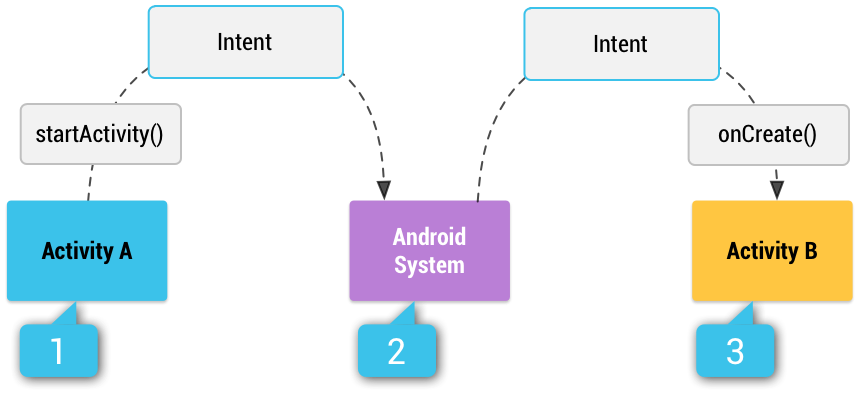
\includegraphics[width=\textwidth]{images/intents/intentresolution.png}
	\caption{Android OS uses filters to pinpoint the set of Activities, Services, and Broadcast receivers that can handle the Intent with help of specified set of action, categories, data scheme associated with an Intent. You will use <intent-filter> element in the manifest file to list down actions, categories and data types associated with any activity, service, or broadcast receiver.}
	\label{fig:intentresolution}
\end{figure}

To allow other apps to start your activity, you need to add an intent-filter element in your manifest file for the corresponding activity element. In order to properly define which intents your activity can handle, each intent filter you add should be as specific as possible in terms of the type of action and data the activity accepts. The system may send a given Intent to an activity if that activity has an intent filter that fulfils the following criteria of the Intent object:

\begin{itemize}
	\item Action : A string naming the action to perform.
	\item Data : A description of the data associated with the intent.
	\item Category: Provides an additional way to characterize the activity handling the intent, usually related to the user gesture or location from which it's started.
\end{itemize}

For example, here's an activity declaration with an intent filter to receive an ACTION\_SEND intent when the data type is text:

\begin{xml}
<activity android:name="ShareActivity">
	<intent-filter>
		<action android:name="android.intent.action.SEND"/>
		<category android:name="android.intent.category.DEFAULT"/>
		<data android:mimeType="text/plain"/>
	</intent-filter>
</activity>
\end{xml}

\section{Broadcastreceiver}
So far, you’ve looked at using Intents to start new application components, but you can also use Intents to broadcast messages anonymously between components via the sendBroadcast() method. As a system-level message-passing mechanism, Intents are capable of sending structured messages across process boundaries. As a result, you can implement Broadcast Receivers to listen for, and respond to, these Broadcast Intents within your applications.

Within your application, construct the Intent you want to broadcast and call sendBroadcast() to send it. Set the action, data, and category of your Intent in a way that lets Broadcast Receivers accurately determine their interest.

\subsection{Receiving a broadcast (without the manifest)}
To receive such a broadcast in an activity (or a fragment), you will need to do four
things.

\begin{enumerate}
	\item you will need to create an instance of your own subclass of
	BroadcastReceiver . The only method you need to (or should) implement is
	onReceive() , which will be passed the Intent that was broadcast, along with a
	Context object that, in this case, you will typically ignore. 
	\item Second, you will need to create an instance of an IntentFilter object, describing
	the sorts of broadcasts you want to receive. Most of these filters are set up to watch
	for a single broadcast Intent action.
	\item You will need to call registerReceiver() , typically from onStart() or onResume() of your
	activity or fragment, supplying your BroadcastReceiver and your IntentFilter .
	\item You will need to call unregisterReceiver() , typically from onStop() or onPause() of your
	activity or fragment, supplying the same BroadcastReceiver instance you provided
	to registerReceiver() .
\end{enumerate}

\subsection{Receiving a broadcast (with the manifest)}
You can also tell Android about broadcasts you wish to receive by adding a
<receiver> element to your manifest, identifying the class that implements your
BroadcastReceiver (via the android:name attribute), plus an <intent-filter> that
describes the broadcast(s) you wish to receive:

\begin{xml}
<receiver android:name=".OnBootReceiver">
	<intent-filter>
		<action android:name="android.intent.action.BOOT_COMPLETED"/>
	</intent-filter>
</receiver
\end{xml}
The good news is that this BroadcastReceiver will be available for broadcasts
occurring at any time. There is no assumption that you have an activity already
running that called registerReceiver() .
The bad news is that the instance of the BroadcastReceiver used by Android to
process a broadcast will live for only so long as it takes to execute the onReceive()
method. At that point, the BroadcastReceiver is discarded. Hence, it is not safe for
a manifest-registered BroadcastReceiver to do anything that needs to run after onReceive()
itself completes, such as forking a thread. After all, Android may well
terminate the process within milliseconds, if there is no other running component
in the process. Moreover, onReceive() is called on the main application thread and may freeze your UI.


\section{Example}
\begin{example}
We will have a good look into the onBoot project from \cite{murphymarkl.2017}: A popular request is to have code get control when the device is powered on. This is
doable but somewhat dangerous, in that too many on-boot requests slow down the
device startup and may make things sluggish for the user.
\end{example}

\begin{example}
	There is an ACTION\_BATTERY\_CHANGED Intent that gets broadcast as the battery
	status changes, both in terms of charge (e.g., 80\% charged) and charging (e.g., the
	device is now plugged into AC power). You simply need to register to receive this
	Intent when it is broadcast, then take appropriate steps. See the full code in \cite{murphymarkl.2017}.
\end{example}


